\documentclass[11pt,compress,t,notes=noshow, xcolor=table]{beamer}
\usepackage[]{graphicx}\usepackage[]{color}
% maxwidth is the original width if it is less than linewidth
% otherwise use linewidth (to make sure the graphics do not exceed the margin)
\makeatletter
\def\maxwidth{ %
  \ifdim\Gin@nat@width>\linewidth
    \linewidth
  \else
    \Gin@nat@width
  \fi
}
\makeatother

\newcommand{\citebutton}[2]{%
\beamergotobutton{\href{#2}{#1}}%
}

\newcommand{\blu}[1]{\textcolor{blue}{#1}}
\newcommand{\org}[1]{\textcolor{orange}{#1}}
\newcommand{\ques}{\textbf{\textcolor{red}{Question:  }}}
\newcommand{\questionssofar}{\begin{frame}\frametitle{Any questions?}\end{frame}}

\newcommand\warning{%
 \makebox[1.4em][c]{%
 \makebox[0pt][c]{\raisebox{.1em}{\scriptsize!}}%
 \makebox[0pt][c]{\color{red}\normalsize$\bigtriangleup$}}}%

\definecolor{fgcolor}{rgb}{0.345, 0.345, 0.345}
\newcommand{\hlnum}[1]{\textcolor[rgb]{0.686,0.059,0.569}{#1}}%
\newcommand{\hlstr}[1]{\textcolor[rgb]{0.192,0.494,0.8}{#1}}%
\newcommand{\hlcom}[1]{\textcolor[rgb]{0.678,0.584,0.686}{\textit{#1}}}%
\newcommand{\hlopt}[1]{\textcolor[rgb]{0,0,0}{#1}}%
\newcommand{\hlstd}[1]{\textcolor[rgb]{0.345,0.345,0.345}{#1}}%
\newcommand{\hlkwa}[1]{\textcolor[rgb]{0.161,0.373,0.58}{\textbf{#1}}}%
\newcommand{\hlkwb}[1]{\textcolor[rgb]{0.69,0.353,0.396}{#1}}%
\newcommand{\hlkwc}[1]{\textcolor[rgb]{0.333,0.667,0.333}{#1}}%
\newcommand{\hlkwd}[1]{\textcolor[rgb]{0.737,0.353,0.396}{\textbf{#1}}}%
\let\hlipl\hlkwb

\usepackage{framed}
\makeatletter
\newenvironment{kframe}{%
 \def\at@end@of@kframe{}%
 \ifinner\ifhmode%
  \def\at@end@of@kframe{\end{minipage}}%
  \begin{minipage}{\columnwidth}%
 \fi\fi%
 \def\FrameCommand##1{\hskip\@totalleftmargin \hskip-\fboxsep
 \colorbox{shadecolor}{##1}\hskip-\fboxsep
     % There is no \\@totalrightmargin, so:
     \hskip-\linewidth \hskip-\@totalleftmargin \hskip\columnwidth}%
 \MakeFramed {\advance\hsize-\width
   \@totalleftmargin\z@ \linewidth\hsize
   \@setminipage}}%
 {\par\unskip\endMakeFramed%
 \at@end@of@kframe}
\makeatother

\definecolor{shadecolor}{rgb}{.97, .97, .97}
\definecolor{messagecolor}{rgb}{0, 0, 0}
\definecolor{warningcolor}{rgb}{1, 0, 1}
\definecolor{errorcolor}{rgb}{1, 0, 0}
\newenvironment{knitrout}{}{} % an empty environment to be redefined in TeX

\usepackage{alltt}
\newcommand{\SweaveOpts}[1]{}  % do not interfere with LaTeX
\newcommand{\SweaveInput}[1]{} % because they are not real TeX commands
\newcommand{\Sexpr}[1]{}       % will only be parsed by R
\newcommand{\xmark}{\ding{55}}%


\usepackage[english]{babel}
\usepackage[utf8]{inputenc}

\usepackage{dsfont}
\usepackage{verbatim}
\usepackage{amsmath}
\usepackage{amsfonts}
\usepackage{amssymb}
\usepackage{bm}
\usepackage{csquotes}
\usepackage{multirow}
\usepackage{longtable}
\usepackage{booktabs}
\usepackage{enumerate}
\usepackage[absolute,overlay]{textpos}
\usepackage{psfrag}
\usepackage{algorithm}
\usepackage{algpseudocode}
\usepackage{eqnarray}
\usepackage{arydshln}
\usepackage{tabularx}
\usepackage{placeins}
\usepackage{tikz}
\usepackage{setspace}
\usepackage{colortbl}
\usepackage{mathtools}
\usepackage{wrapfig}
\usepackage{bm}
\usepackage{amsmath}
\usepackage{pifont}

\usetikzlibrary{shapes.multipart,shapes,arrows,automata,positioning,calc,chains,trees, shadows}
\tikzset{
  %Define standard arrow tip
  >=stealth',
  %Define style for boxes
  punkt/.style={
    rectangle,
    rounded corners,
    draw=black, very thick,
    text width=6.5em,
    minimum height=2em,
    text centered},
  % Define arrow style
  pil/.style={
    ->,
    thick,
    shorten <=2pt,
    shorten >=2pt,}
}

\tikzstyle{vec}=[draw, rectangle, fill = white, minimum width=5mm, minimum height=1cm, inner sep = 2pt]

\usepackage{subfig}

% Defines macros and environments
\usepackage{../../style/lmu-lecture}


\let\code=\texttt
\let\proglang=\textsf

\setkeys{Gin}{width=0.9\textwidth}

\setbeamertemplate{frametitle}{\expandafter\uppercase\expandafter\insertframetitle}

\usepackage{bbm}
% basic latex stuff
\newcommand{\pkg}[1]{{\fontseries{b}\selectfont #1}} %fontstyle for R packages
\newcommand{\lz}{\vspace{0.5cm}} %vertical space
\newcommand{\dlz}{\vspace{1cm}} %double vertical space
\newcommand{\oneliner}[1] % Oneliner for important statements
{\begin{block}{}\begin{center}\begin{Large}#1\end{Large}\end{center}\end{block}}


%new environments
\newenvironment{vbframe}  %frame with breaks and verbatim
{
 \begin{frame}[containsverbatim,allowframebreaks]
}
{
\end{frame}
}

\newenvironment{vframe}  %frame with verbatim without breaks (to avoid numbering one slided frames)
{
 \begin{frame}[containsverbatim]
}
{
\end{frame}
}

\newenvironment{blocki}[1]   % itemize block
{
 \begin{block}{#1}\begin{itemize}
}
{
\end{itemize}\end{block}
}

\newenvironment{fragileframe}[2]{  %fragile frame with framebreaks
\begin{frame}[allowframebreaks, fragile, environment = fragileframe]
\frametitle{#1}
#2}
{\end{frame}}


\newcommand{\myframe}[2]{  %short for frame with framebreaks
\begin{frame}[allowframebreaks]
\frametitle{#1}
#2
\end{frame}}

\newcommand{\remark}[1]{
  \textbf{Remark:} #1
}


\newenvironment{deleteframe}
{
\begingroup
\usebackgroundtemplate{
\includegraphics[width=\paperwidth,height=\paperheight]{../style/color/red.png}}
 \begin{frame}
}
{
\end{frame}
\endgroup
}
\newenvironment{simplifyframe}
{
\begingroup
\usebackgroundtemplate{
\includegraphics[width=\paperwidth,height=\paperheight]{../style/color/yellow.png}}
 \begin{frame}
}
{
\end{frame}
\endgroup
}\newenvironment{draftframe}
{
\begingroup
\usebackgroundtemplate{
\includegraphics[width=\paperwidth,height=\paperheight]{../style/color/green.jpg}}
 \begin{frame}
}
{
\end{frame}
\endgroup
}
% https://tex.stackexchange.com/a/261480: textcolor that works in mathmode
\makeatletter
\renewcommand*{\@textcolor}[3]{%
  \protect\leavevmode
  \begingroup
    \color#1{#2}#3%
  \endgroup
}
\makeatother





\input{../../latex-math/basic-math.tex}
\input{../../latex-math/basic-ml.tex}

\newcommand{\titlefigure}{figure/gpt2-title.png}
\newcommand{\learninggoals}{
\item 
Understand language models as universal task solvers
\item Understand the implications of such models}

\title{Generative Pre-Trained Transformers}
% \author{}
\institute{\href{https://slds-lmu.github.io/lecture_dl4nlp/}{slds-lmu.github.io/lecture\_dl4nlp}}
\date{}

\begin{document}
\lecturechapter{GPT-2 (2019)}
\lecture{Deep Learning for NLP}

% ------------------------------------------------------------------------------

\begin{frame}{Starting with a controversy}

\vfill

\begin{figure}
\centering
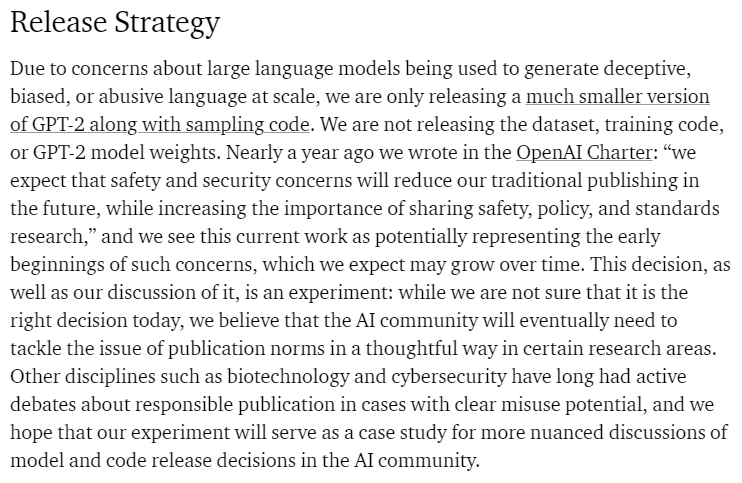
\includegraphics[width = 9cm]{figure/72-gpt2-release.png}\\ 
\citebutton{Source: OpenAI Blog}{https://openai.com/research/better-language-models}
\end{figure}

\vfill

\end{frame}

% ------------------------------------------------------------------------------

\begin{frame}{Capabilities -- Storytelling}

\vfill

\begin{figure}
\centering
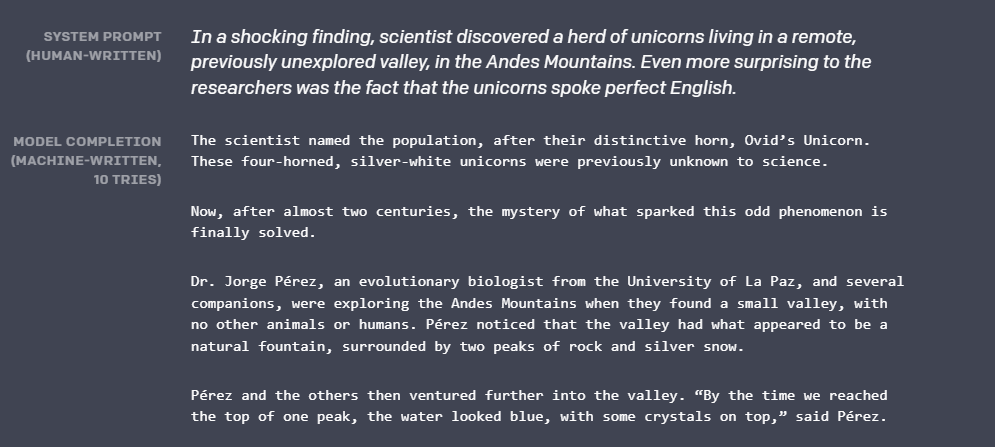
\includegraphics[width = 11cm]{figure/72-gpt2-story.png}\\ 
\citebutton{Source: OpenAI Blog}{https://openai.com/research/better-language-models}
\end{figure}

\vfill

\end{frame}

% ------------------------------------------------------------------------------

\begin{frame}{Capabilities -- Storytelling}

\vfill

\begin{figure}
\centering
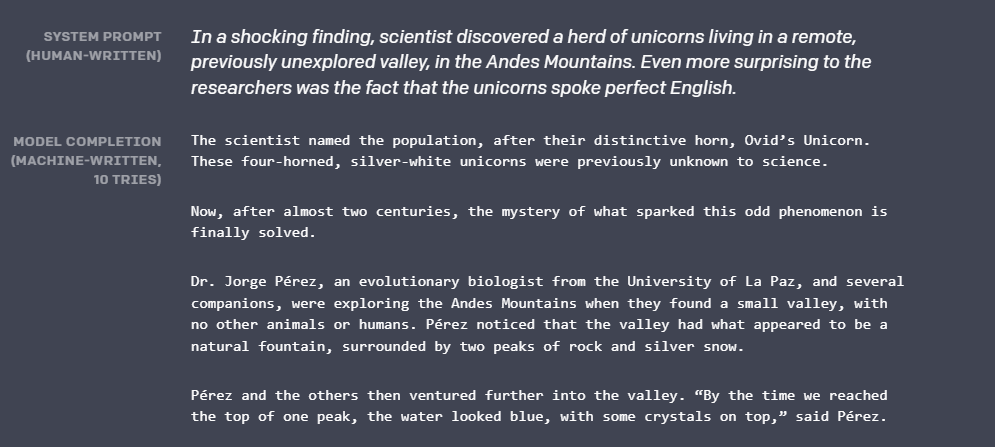
\includegraphics[width = 6cm]{figure/72-gpt2-story.png}\\ 
\citebutton{Source: OpenAI Blog}{https://openai.com/research/better-language-models}
\end{figure}

\begin{itemize}
	\item \textbf{In 2019:} Great achievement as the model is able to continue a made up story \textit{in a coherent way} by making up its own facts
	\item[] Sill: Not very consistent (``\texttt{four-horned [...] unicorns}``)
	\item \textbf{In 2023:} Nowadays this phenomenon is known as \textbf{hallucination} and a lot of research effort is put into mitigating this behaviour
\end{itemize}

\vfill

\end{frame}

% ------------------------------------------------------------------------------

\begin{frame}{The architecture}

\vfill

\begin{itemize}
	\item Transformer decoder pre-trained on AR language modeling
	\item Custom web scrape (not publicly available) of all outbound links from Reddit
	\item[$\to$] 8M documents / 40GB of text
	\item Byte-level BPE for tokenization
	\item Increased context size: $512 \to 1024$
\end{itemize}

\begin{figure}
\centering
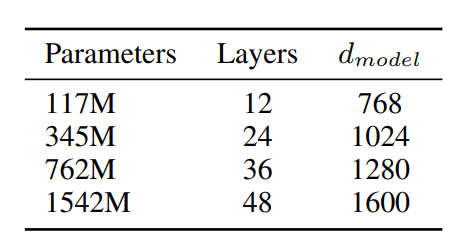
\includegraphics[width = 6cm]{figure/72-gpt2-size.png}\\ 
\citebutton{Source: Radford et al., 2019}{https://openai.com/research/better-language-models}
\end{figure}

\vfill

\end{frame}

% ------------------------------------------------------------------------------

\begin{frame}{Language models as multitask learners}

\vfill

\begin{itemize}

\item[] ``But as exemplified in McCann et al. (2018), language
	provides a flexible way to specify tasks, inputs,
	and outputs all as a sequence of symbols.

\item[] For
	example, a translation training
	example can be written as the sequence (translate to
	french, english text, french text).''
	\item Model benefits from seeing ``natural`` occurrences of task demonstrations during pre-training on large-scale web corpora
	\item[] $\to$ Related rationale to T5 (\textit{literal task descriptions}), but slightly different (\textit{acquired on the fly already during pre-training}).
\end{itemize}

\begin{figure}
\centering
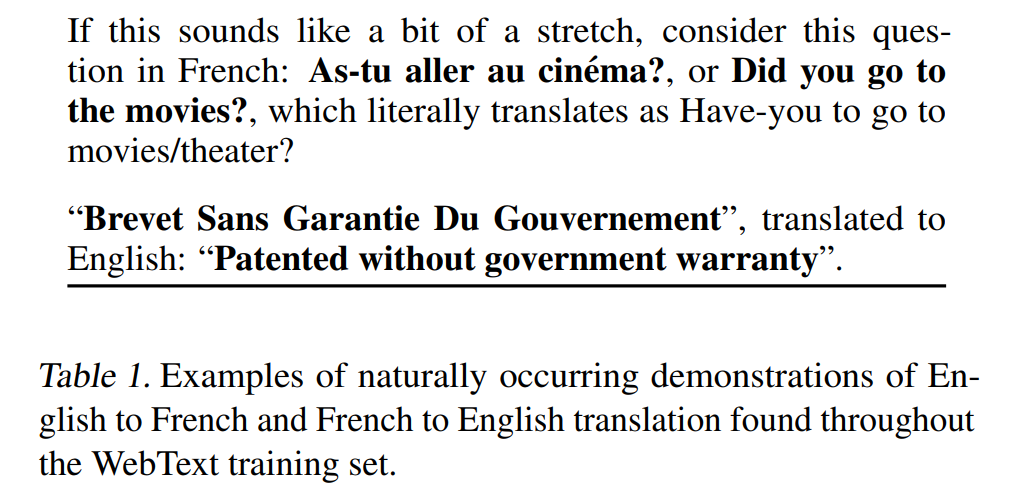
\includegraphics[width = 7cm]{figure/72-gpt2-demo-wild.png}\\ 
\citebutton{Source: Radford et al., 2019}{https://openai.com/research/better-language-models}
\end{figure}

\vfill

\end{frame}

% ------------------------------------------------------------------------------



\begin{frame}{Capabilities -- Zero-Shot}

\vfill

\begin{itemize}
	\item \textit{Zero-shot} refers to solving a task which the model was not previously explicitly trained on, just providing it with a description of the task but no demonstrations, i.e. input/output pairs.
	\item \textit{Few-shot} would be a relaxation of this setting, allowing for also providing the models with demonstrations (but still no training/gradient updates).
	\item Radford et al. show GPT-2's zero-shot capabilities on a range of different tasks, paving the way for the developments that came with GPT-3.
\end{itemize}

\vfill

\end{frame}

% ------------------------------------------------------------------------------

\begin{frame}{Capabilities -- Zero-Shot}

\vfill

\begin{figure}
\centering
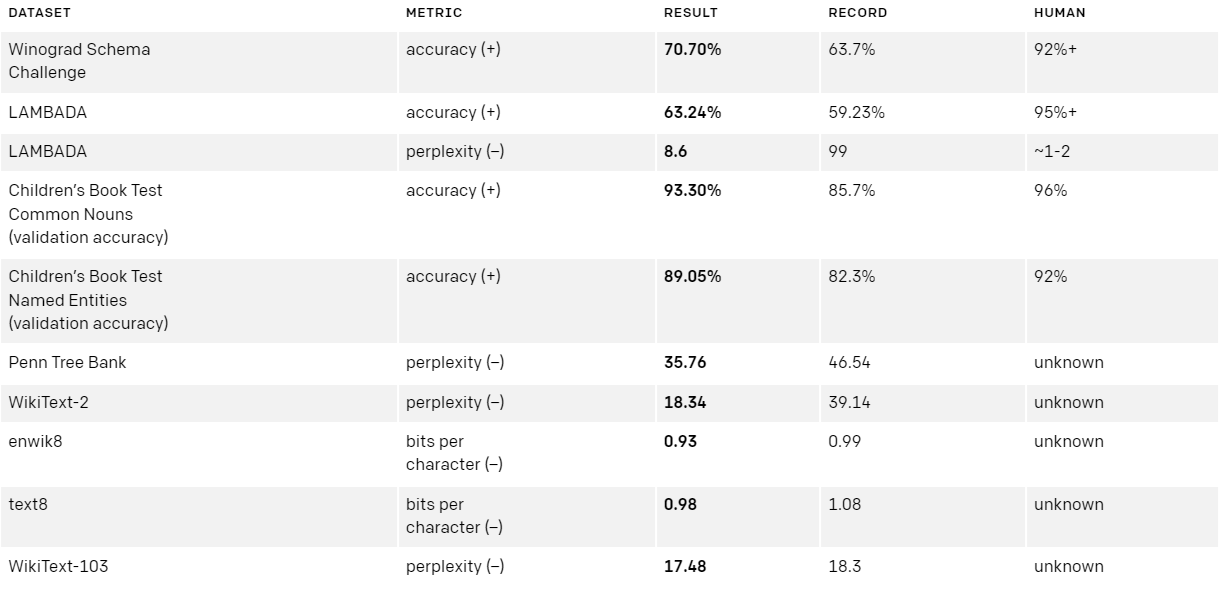
\includegraphics[width = 11cm]{figure/72-gpt2-zeroshot.png}\\ 
\citebutton{Source: Radford et al., 2019}{https://openai.com/research/better-language-models}
\end{figure}

\vfill

\footnotesize{(Note: The numbers correspond to the last row of the Table on slide 6)}

\end{frame}

% ------------------------------------------------------------------------------

\begin{frame}{Capabilities -- Factual knowledge}

\vfill

\textbf{Natural Questions} \citebutton{Kwiatkowski et al., 2019}{https://aclanthology.org/Q19-1026/}

\begin{itemize}
	\item Testing the \textit{factual knowledge} that is present in the pre-trained model
	\item Smallest model (117M): $< 1\%$
	\item GPT-2 (1542M): $4.1\%$
	\item[] $\to$ Model capacity as a major factor
	\item Calibration: High accuracy (63.1\%) on the 1\% most confident answers
\end{itemize}

\vfill

\end{frame}

% ------------------------------------------------------------------------------

\begin{frame}{Capabilities -- Factual knowledge}

\vfill

\textbf{The 30 most confident answers:}

\begin{figure}
\centering
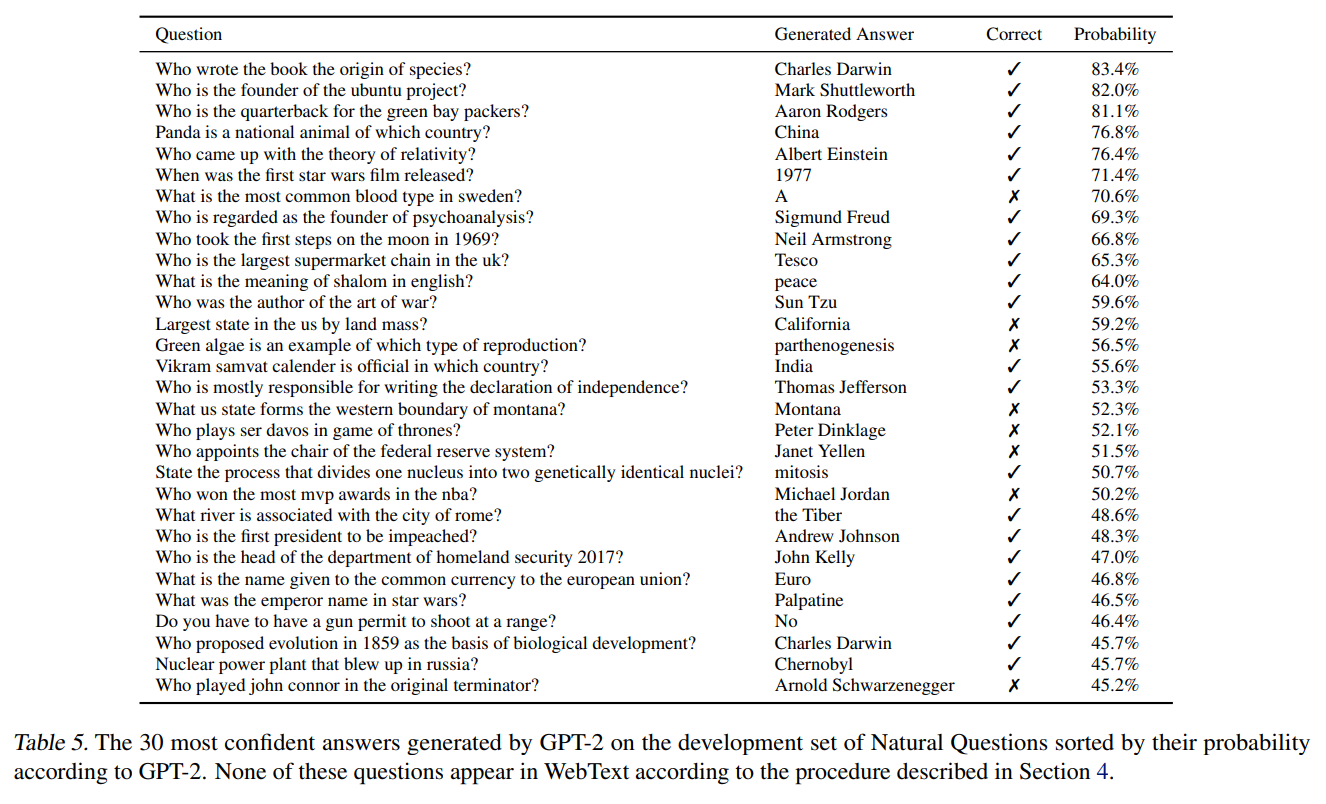
\includegraphics[width = 11cm]{figure/72-gpt2-qa.png}\\ 
\citebutton{Source: Radford et al., 2019}{https://openai.com/research/better-language-models}
\end{figure}

\vfill

\end{frame}

% ------------------------------------------------------------------------------

\begin{frame}{In the meantime}

\vfill

\begin{figure}
\centering
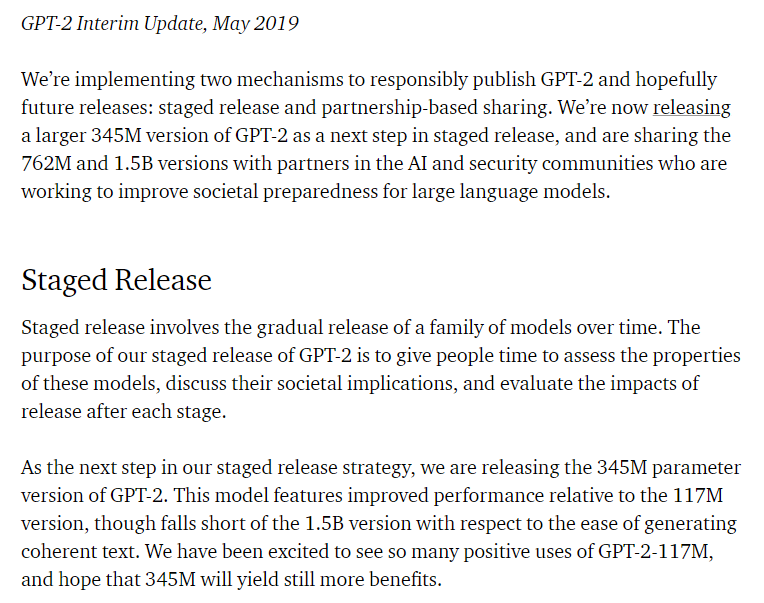
\includegraphics[width = 9cm]{figure/72-gpt2-release2.png}\\ 
\citebutton{Source: OpenAI Blog}{https://openai.com/research/better-language-models}
\end{figure}

\vfill

\end{frame}

% ------------------------------------------------------------------------------

\begin{frame}{In the meantime}

\vfill

\begin{itemize}
	\item Available on huggingface: \url{https://huggingface.co/gpt2}
	\item GPT-3 built on the foundation laid by GPT-2
	\item (also ChatGPT happened)
	\item GPT-2 (multi-task learning) extended to
	GPT-3 (prompting)
%        Prompting models has become more and more common\\ (cf. next chapter)
	\item Few-/Zero-Shot capabilites of models have become more important (cf. next chapter)
	\item Models of over $200\times$ the size of GPT-2 have been trained
	\item Transformer still the backbone of (nearly) all of them
\end{itemize}

\vfill

\end{frame}

% ------------------------------------------------------------------------------

\endlecture
\end{document}
